\chapter{QUENCHING PROCESS}
\section{Experimental targets}
\begin{itemize}
	\item Understand  the  quenching  process:  chosing  heang  temperature,  heang  me  and  cooling environment.
	\item Study the relaonship between quenching temperature, colling rate, and hardness of steel.
\end{itemize}
\section{Theoretical summary}
Tempering is done to develop the required combination of hardness, strength, and toughness or to relieve the brittleness of fully hardened steels. Tempering is the process of reheating the steel at a relatively low temperature leading to precipitation and spheroidization of the carbides present in the microstructure. The tempering temperature and mes are generally controlled to produce the final properties required of the steel. The result is a component with the appropriate combination of hardness,  strength,  and  toughness  for  the  intended  application.  Tempering  is  also  effective  in relieving the stresses induced by quenching.
\paragraph{Low tempering} Ranging from $ 150^\circ$C - $250^\circ$C\\
The  microscopic  structure  after  the  process  is  called mactencite,  the  work piece  hardness  change a little, and receive erosion resistance.
\paragraph{Low tempering} Ranging from $ 300^\circ\text{C}- 450^\circ\text{C}$\\
After the process the hardness of the work piece is high (40-45HRC), stress is lowered by a bit, increase elasticity, yield strength increase to maximum value.
\paragraph{Low tempering} Ranging from $ 500^\circ\text{C} - 650^\circ\text{C}$
\section{Detailed experiment}
\begin{itemize}
	\item 3 samples are quenched in water and then low tempered at $ 250^\circ $C for about 20 minutes
	\item 3 samples are quenched in oil.
\end{itemize}
\section{Measurement results}\clearpage
\begin{landscape}
%	\hfill
	\vspace*{\fill}
	\renewcommand{\arraystretch}{1.5}
	\begin{table}[ht]
		\begin{tabular}[ht]{lrrrrrrrrrrrr}
			\toprule
			\multicolumn{1}{c}{Hardness type} & \multicolumn{4}{c}{Sample 1 (HRC)}  & \multicolumn{4}{c}{Sample 2 (HRC)}  & \multicolumn{4}{c}{Sample 3 (HRC)}\\
			\cmidrule{2-5}\cmidrule{6-9}\cmidrule{10-13} \multicolumn{1}{c}{No} & $ 1 $ & $ 2 $ & $ 3 $ & Avg & $ 4 $ & $ 5 $ & $ 6 $ & Avg & $ 7 $ & $ 8 $ & $ 9 $ & Avg\\\midrule
			\rowcolor{lightgray!20}{\cellcolor[HTML]{C0C0C0}}Before tempering &10.63&10.63&10.20 & 10.49 & 10.90&9.23&11.57&10.57&10.33  &9.93&9.70&9.99\\
			{\cellcolor[HTML]{C0C0C0}}Water &58.50&60.00&60.00&59.50&60.50&59.00&60.30&59.93&57.50&58.00&59.50&58.33\\
			\rowcolor{lightgray!20}{\cellcolor[HTML]{C0C0C0}}Oil &54.00&54.00&51.00&53.00&54.00&54.00&50.00&52.67&53.80&52.50&50.00&52.10\\		{\cellcolor[HTML]{C0C0C0}}Air &14.00&16.00&17.00&15.67&17.00&18.80&19.00&18.27&15.00&14.80&16.00&15.27\\		\rowcolor{lightgray!20}{\cellcolor[HTML]{C0C0C0}}High tempering ($ 550^\circ C $) &36.20&35.20&35.50&35.63&36.10&36.00&36.00&36.03&35.80&36.80&36.90&36.50\\		{\cellcolor[HTML]{C0C0C0}}Low tempering ($ 150^\circ C $) &55.20&57.00&58.00&56.73&54.40&56.30&55.80&55.50&55.00&55.30&54.30&54.87\\\bottomrule
			%		\caption{Measurement Results}
		\end{tabular}
		\caption{Measurement results}
	\end{table}
	
	\vspace*{\fill}
\end{landscape}
\section{Relationship}
\begin{figure}[ht]
	\centering
	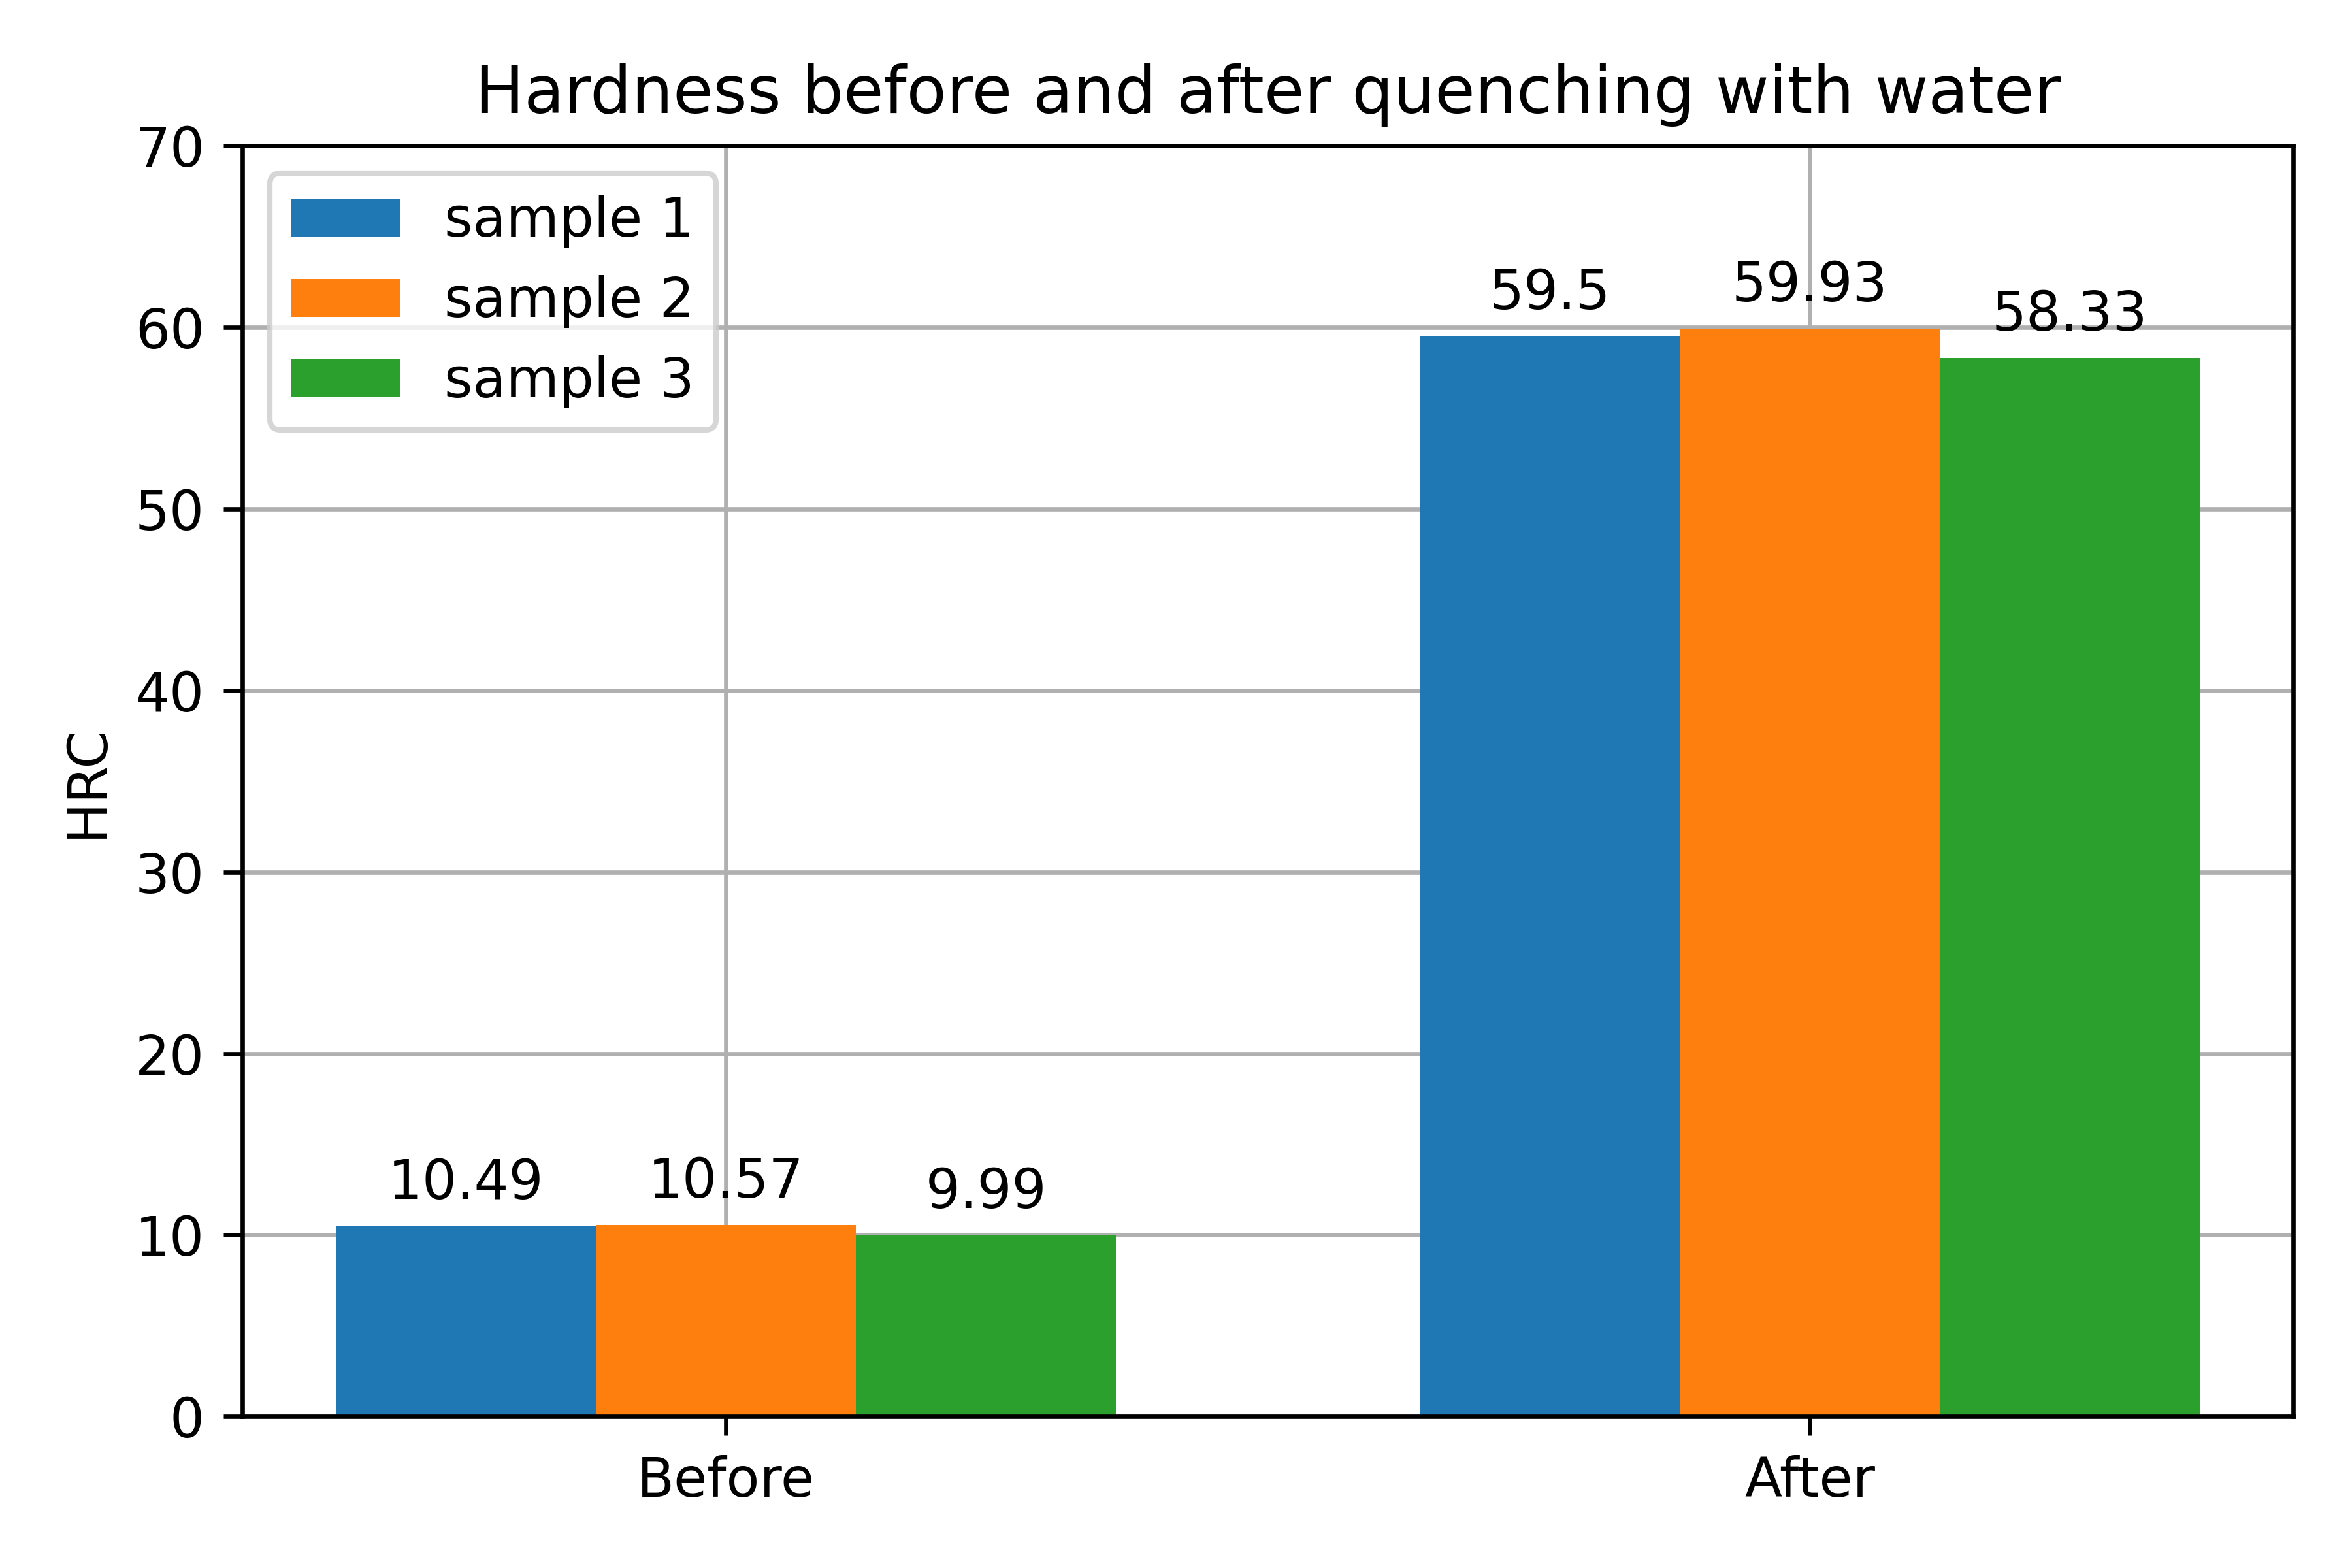
\includegraphics[width=150mm]{Hardness.png}
	\caption{The relationship of hardness between before and after quenching}
\end{figure}
\begin{figure}[ht]
	\centering
	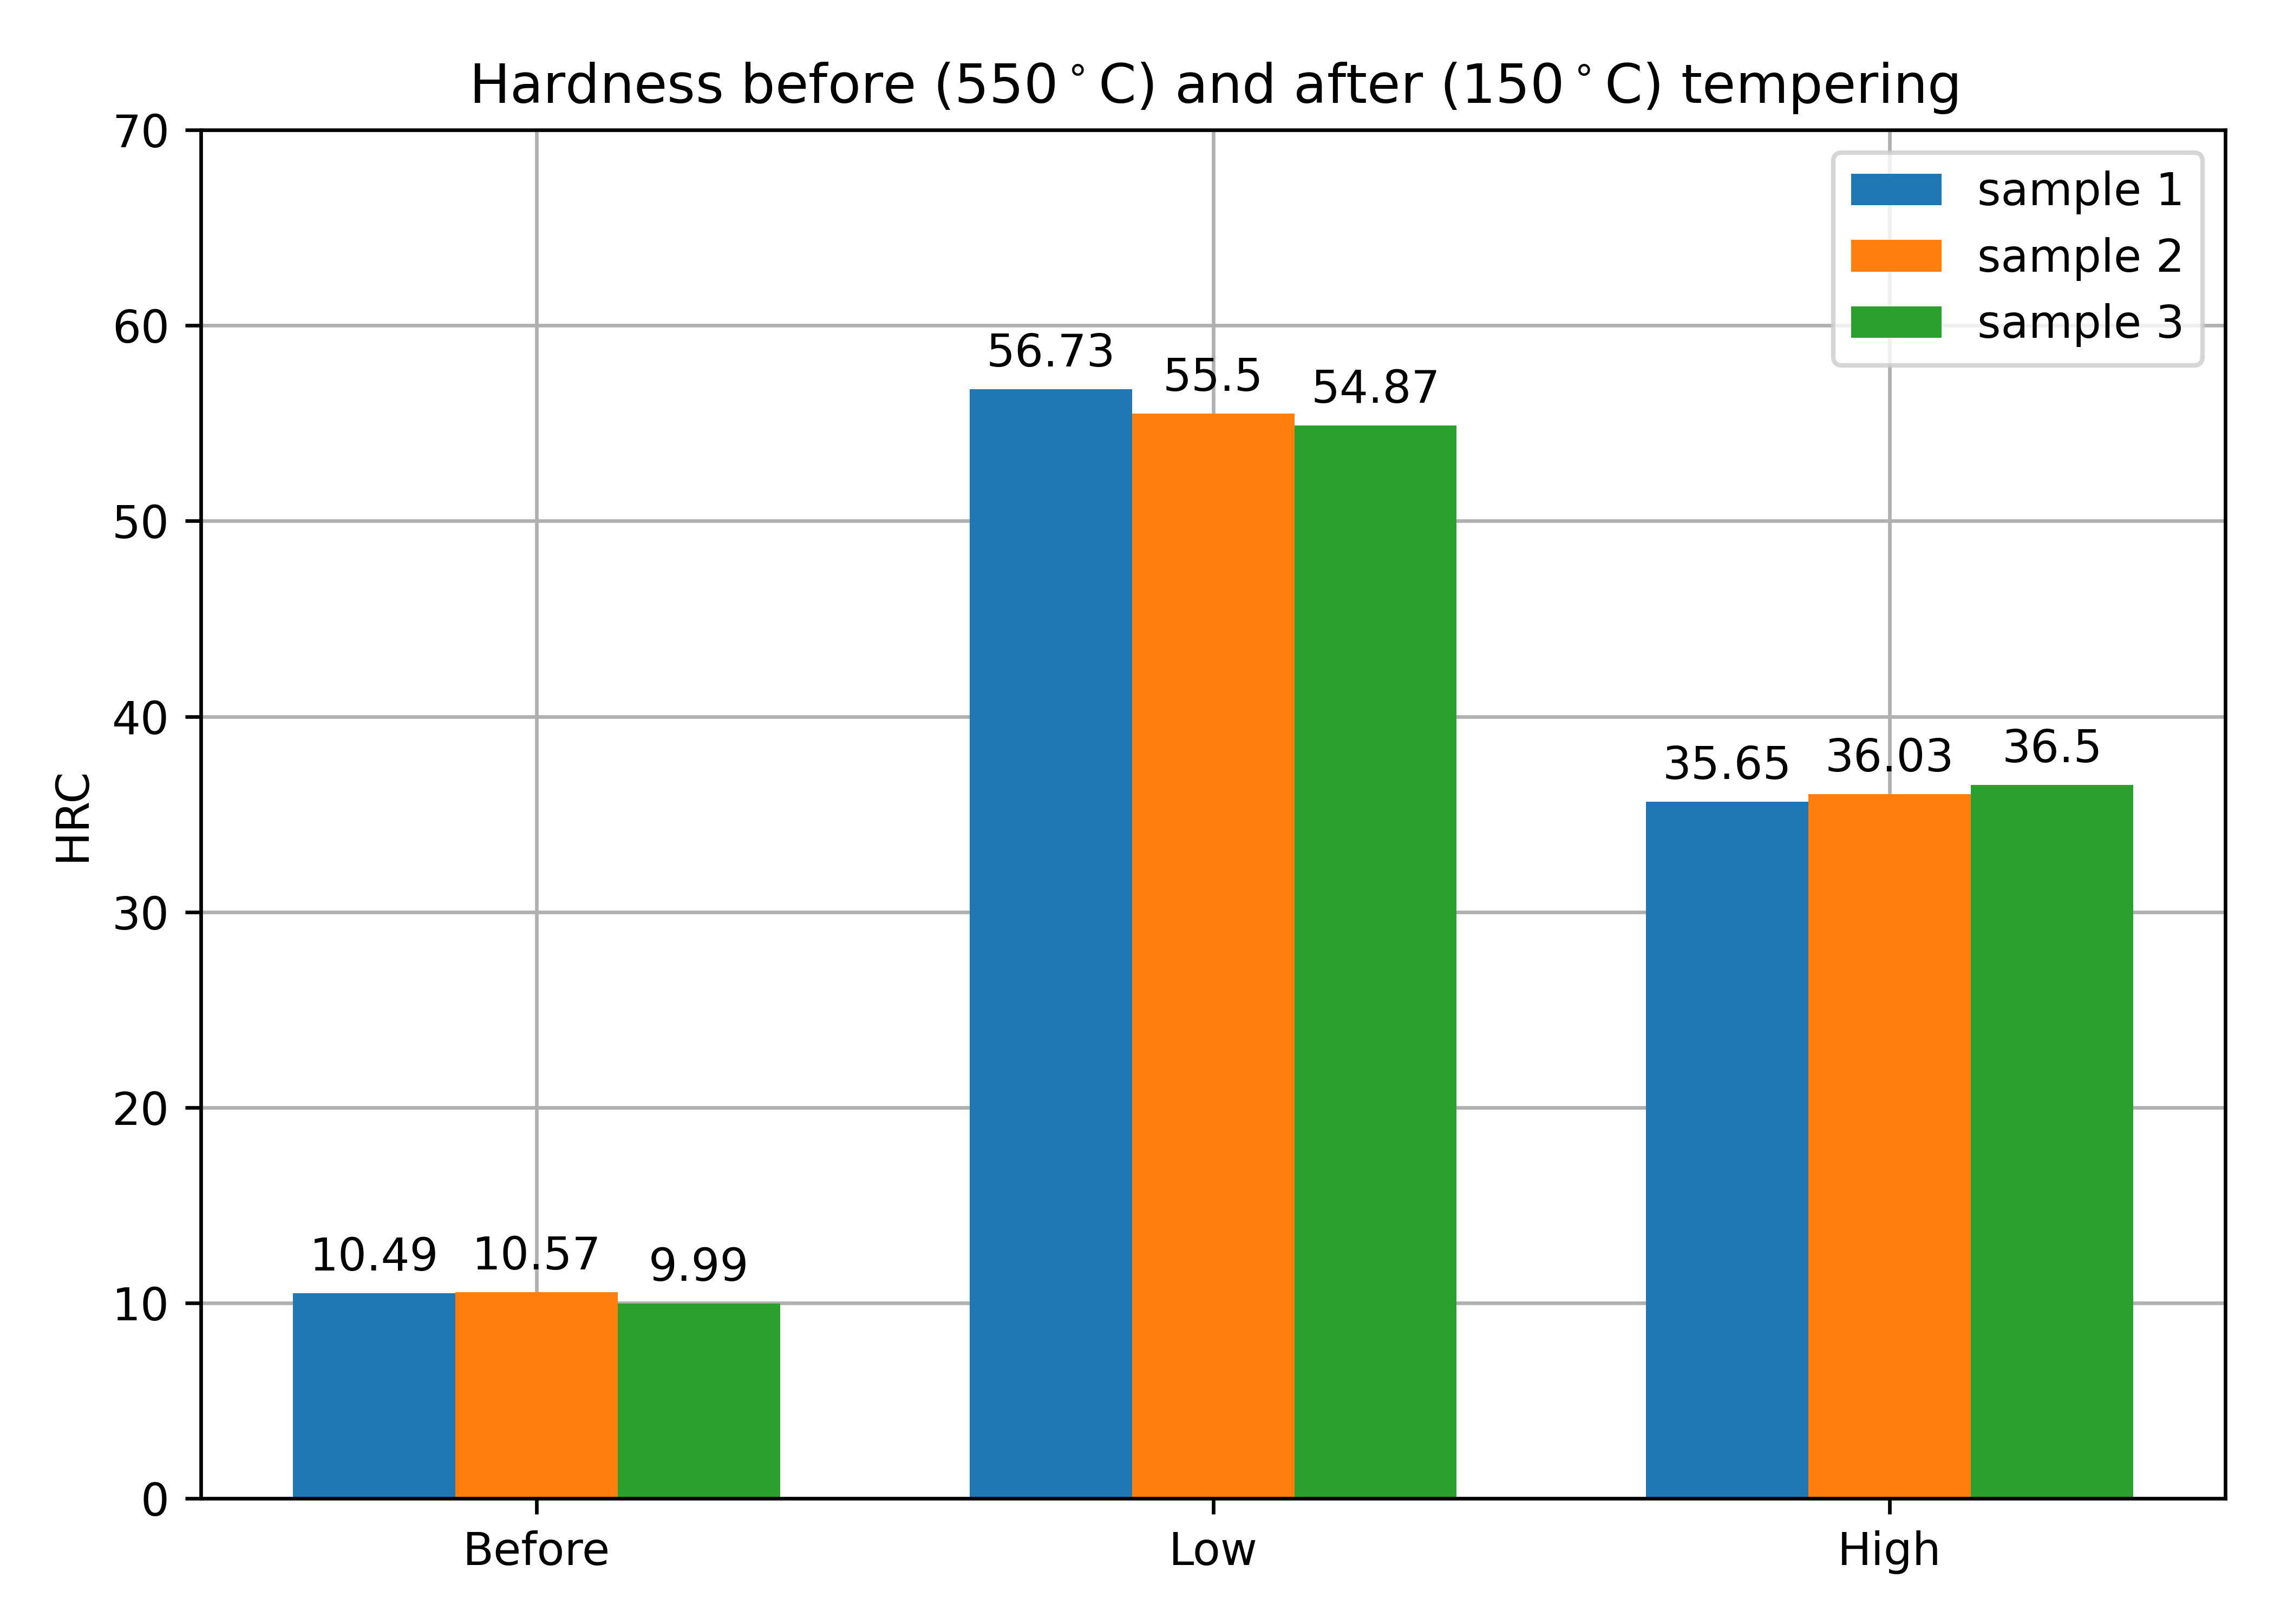
\includegraphics[width=150mm]{Hardness2.png}
	\caption{The relationship of hardness after tempering}
	\label{label}
\end{figure}
\section{Conclusion}
\begin{itemize}
	\item After tempering, the hardness of the sample in the experiment increased. The hardness of the sample increases gradually as it cools in the environment in the order of air, oil, and water. At the same heating temperature and incubation time and furnace when cooled at different field conditions, the samples received have different hardness (increase or decrease).
	\item Test samples after quenching at high temperatures have lower hardness than when quenching at low temperatures.
	\item After quenching the sample has been tempered, the hardness of the sample decreases, but depends on the quenching temperature and required hardness after quenching.
	\item After quenching the sample has been tempered, the hardness of the sample decreases, but depends on the quenching temperature and required hardness after quenching.
\end{itemize}